\chapter{Entwicklung und Implementation}

\section{Aufbau und Aufbereitung des Datensatzes}
\subsection{Rohvideos}

Der Datensatz basiert auf einer eigens erstellten Sammlung von Videoaufnahmen der deutsche Gebärdensprache (DGS) und wurde speziell für die Klassifikation statischer Fingeralphabetzeichen konzipiert. Die Rohvideos wurden manuell aufgezeichnet und liegen im MP4-Format vor.

Die Benennungskonvention der Videodateien lautet \texttt{alph\_[og|fw]\_[Label][Nummer].mp4}, wobei \texttt{[og|fw]} den aufzeichnenden protokolliert, \texttt{[Label]} das jeweilige Fingersprachezeichen und \texttt{[Nummer]} die fortlaufende Nummer innerhalb eines Labels spezifiziert. Die Speicherung erfolgt im Verzeichnis \texttt{ml\_pipeline/resources/videos\_prototype/}.

Der Datensatz umfasst 226 Rohvideos, die auf 26 Klassen verteilt sind. Die Klassenauswahl beschränkt sich auf die 24 statischen Buchstaben A–Y (ohne J und Z, da diese dynamische Handbewegungen erfordern und somit mit dem statischen Ansatz des Klassifikators nicht kompatibel sind), das Sonderzeichen SCH sowie die Leerklasse NONE, die die Unbestimmtheit des Ergebnisses darstellt. Die Anzahl der Originaufnahmen pro Klasse variiert zwischen 3 und 5, wobei 16 Klassen mit je 5, 8 Klassen mit je 4 und 2 Klassen (F, NONE) mit je 3 Aufnahmen vertreten sind.

\subsection{Frame-Extraktion und Handdetektion}

\#TODO MediaPipe Hand/Palm Detection

Zur Verarbeitung der Rohvideos wird jeder Einzelrahmen (Frame) mittels OpenCV Videocapture einzeln extrahiert und ohne vorherige Vorfilterung der Erkennungspipeline zugeführt.

Die Hand-Erkennung und Landmark-Extraktion erfolgt mithilfe des MediaPipe-Handdetektors (Lugaresi et al., 2019) in der Konfiguration für statische Bildanalyse mit einer maximalen Detektionskapazität von 2 Händen pro Frame und einer Mindestkonfidenz von 70. Pro Hand werden 21 Landmarks extrahiert, die den Handgelenkspunkt (WRIST) sowie die Gelenke der fünf Finger (Daumen: CMC, MCP, IP, TIP; Indexfinger: MCP, PIP, DIP, TIP; Mittelfinger: MCP, PIP, DIP, TIP; Ringfinger: MCP, PIP, DIP, TIP; Kleinfinger: MCP, PIP, DIP, TIP) umfassen.


\subsection{Augmentation}

Die Augmentationspipeline wendet sequenziell Transformationen auf die extrahierten Landmarks an. Jeder Schritt kann mehrere Variationen erzeugen, die kumulativ kombiniert werden:

Die Extrahierte Gesten Daten werden im folgenden schritt mittels Augmentation vervielfacht und gegen Overfitting angepasst. Die Augmentationspipeline bietet  die folgenden Augmentationsoptionen:
- Translate: addiert einen Offset auf die Gesture Datem
- Spiegelung: Spiegelt gesten horizontal
- Scale: scaliert die gesten
- Jitter: Fügt der Geste zufälige individuelle  Fehler hinzu
- Zoom: Zufälliger zoom der Geste
- DropFrames: Skips frames in order to simulate missing Frames
Für die verwendeten Optionen sind:
- Mirror
- 2xTranslation
- 5xZoom

\#TODO Pickle Inspect Gegenüberstellung der Gesten nach Augmentation

\subsection{Normalisierung und Interpolation}

Die extrahierten Landmarks werden für eine effiziente und positionsinvariante Darstellung normalisiert. Hierbei werden alle Landmark-Koordinaten relativ zum Handgelenk positioniert und in den int16-Zahlenbereich ({-}32.768 bis 32.767) umgerechnet. Die Landmark-Daten werden als Dictionary mit den 21 benannten Schlüsseln und den zugehörigen \([x, y, z]\)-Koordinaten abgebildet. Zusätzlich wird die absolute Handgelenkposition (\texttt{wrist\_pos}) in Skalierung auf den int16-Bereich sowie die Bounding-Box der Hand in Pixelkoordinaten (\texttt{hand\_area}) gespeichert. Die absoluten Landmark-Positionen in Pixelkoordinaten (\texttt{landmark\_pos}) werden ebenfalls erfasst.

Für eine einheitliche Darstellung aller Sequenzen erfolgt eine FPS-Normalisierung auf 60\,FPS mittels linearer Interpolation zwischen den Frames. Frames, in denen eine Hand nicht erkannt wird, werden durch leere Handstrukturen mit der Sentinel-Koordinate \([{-100}, {-100}]\) repräsentiert und bei der Interpolation als Sprungpunkte behandelt.

\subsection{Datenstrukturen und Speicherung}

Die verarbeiteten Geste- und Handdaten werden in den folgenden Datenstrukturen abgebildet:

\paragraph{Gesture} -- Repräsentation einer vollständigen Geste-Sequenz:
\begin{itemize}
    \item \texttt{label}: Klasse der Geste (str)
    \item \texttt{fps}: Aktuelle Bildwiederholrate (float)
    \item \texttt{frames}: Liste von Frames, wobei jeder Frame eine Liste von zwei Hand-Objekten \texttt{[left, right]} enthält
\end{itemize}

\paragraph{Hand} -- Darstellung einer einzelnen Hand in einem Frame (frozen dataclass):
\begin{itemize}
    \item \texttt{left\_hand}: Seitenzugehörigkeit (bool)
    \item \texttt{wrist\_pos}: Absolute Handgelenkposition in int16-Skalierung \texttt{[x, y]}
    \item \texttt{landmarks}: Dictionary mit 21 benannten Landmarks relativ zum Handgelenk
    \item \texttt{hand\_area}: Bounding-Box in Pixelkoordinaten \texttt{(x, y, width, height)}
    \item \texttt{landmark\_pos}: Absolute Landmark-Positionen in Pixelkoordinaten (21 $\times$ \texttt{[x, y]})
\end{itemize}

Die verarbeiteten Geste-Daten werden im Pickle-Format (\texttt{.pkl}) abgelegt. Der Dateiname folgt dem Muster \texttt{\{Label\}\_\{Augmentierungstyp\}\_\{UUID\}.pkl}, wobei die UUID die ersten vier Hexadezimalzeichen eines UUID4 darstellt. Die Speicherung erfolgt im Verzeichnis \texttt{resources/gestures/}. Die Verarbeitung der Videodateien und die Speicherung der Ergebnisse werden mittels Multiprocessing unter Auslastung von 80\,\% der verfügbaren CPU-Kerne parallelisiert.

\section{Entwicklung und Training des Klassifikationsmodells}
\subsection{Problemdefinition}

Das zu entwickelnde Modell soll die Fähigkeit besitzen, Gesten bestimmten Gruppen zuzuordnen. Eine Gruppe entspricht dabei immer einer Geste. Diese Einteilung von Datenpunkten (Gesten) in vordefinierte Klassen (Gebärdenalphabet-Zeichen) beschreibt Klassifikationsmodelle. Für jede Geste sollen die Wahrscheinlichkeiten für die zuzuordnenden Klassen ausgegeben werden.

Es liegt keine Binäreklassifikation vor, da mehr als zwei Klassen zu unterscheiden sind. Mit den 26 Klassen (NONE, A–Y ohne J und Z, SCH) handelt es sich um eine Multiklassen-Klassifikation.

\subsection{Datenanalyse}

\paragraph{Input-Format:} Der Klassifikator empfängt einen 88-dimensionalen Feature-Vektor. Dieser setzt sich nach Ausgabe des Hand-Landmark Modells aus 44 Werten für die linke Hand (22 Gelenke $\times$ 2 Koordinaten) und 44 Werten für die rechte Hand (22 Gelenke $\times$ 2 Koordinaten) zusammen.

Die 22 Gelenke pro Hand umfassen die 21 MediaPipe-Landmarks sowie die absolute Handgelenkposition. Koordinaten werden wrist-relativ normalisiert und auf den int16-Bereich ({-}32.768 bis 32.767) skaliert.

\paragraph{Klassenverteilung:} Der Datensatz umfasst 26 Klassen: NONE (Index 0) für Keine Hand erkannt, A--Y (Indizes 1--24) für 24 statische Buchstaben (J und Z ausgeschlossen, da diese dynamische Handbewegungen erfordern) sowie SCH (Index 25) als Sonderzeichen. Die Klassenverteilung ist leicht ungleichmäßig (16 Klassen mit 185, 8 Klassen mit 148, NONE mit 111, F mit 110 Dateien).

\paragraph{Normalisierung:} Alle Koordinaten werden durch den Maximalwert des int16-Bereichs (POS\_MAX = 32.767) dividiert, sodass die Werte im Bereich \([{-}1, 1]\) liegen.

\subsection{Modellauswahl}

Für die Modellauswahl wurden verschiedene Ansätze evaluiert, wobei die Anforderungen des Embedded-Systems (schnelle Inferenz, kleine Modellgröße) und die Input-Struktur (88D-feature-Vektor aus MediaPipe-Landmarks) im Vordergrund standen.

Ein mehrschichtiges Perceptron (MLP) wurde als geeignetstes Modell
identifiziert. Die Input-Struktur war dafür Ausschlaggebend. Die MediaPipe wandelt die räumliche Information der Hand in strukturierte Landmarks um. Daher ist eine convolutionale
Verarbeitung (CNN) unnötig. Studien belegen, dass CNNs bei
Landmark-basiertem Input keine signifikanten Genauigkeitsvorteile
gegenüber MLPs aufweisen. (Fritz, 2025)

Random Forest und SVM wurden ebenfalls in Betracht gezogen, erreichen jedoch in der Literatur geringere Genauigkeiten (70–75\% bzw. 61–76\%) bei vergleichbaren Tasks. Zudem fehlen beiden Modellen nativ kalibrierte Wahrscheinlichkeiten: Random Forest gibt nur harte Klassifikationen aus, während SVM ein zusätzliches Platt-Scaling für Wahrscheinlichkeiten erfordert. (Rahman et al., 2025). Es ist anzumerken das SVM und Random forest auf einer anderen Datenbasis (Photoplethysmography (PPG)) trainiert worden sind.

Das MLP erfüllt die Anforderungen an Ressourcenbeschränkungen und Echtzeitfähigkeit. Die Softmax-Ausgabeschicht liefert direkt kalibrierte Klassenwahrscheinlichkeiten, die für die nachfolgende Verarbeitung benötigt werden. Während direkte Quantisierung zu Genauigkeitsverlust führen kann, zeigen Studien, dass INT8-Quantisierung bei MLP-Modellen mit geeigneten Techniken (LayerNorm, Kalibrierung) Verluste von unter 1\% erreicht. Ein akzeptabler Kompromiss für den Embedded-Einsatz (blogdeveloperspot, 2025).

\subsection{Modellarchitektur}

\begin{figure}[!htbp]
    \centering
    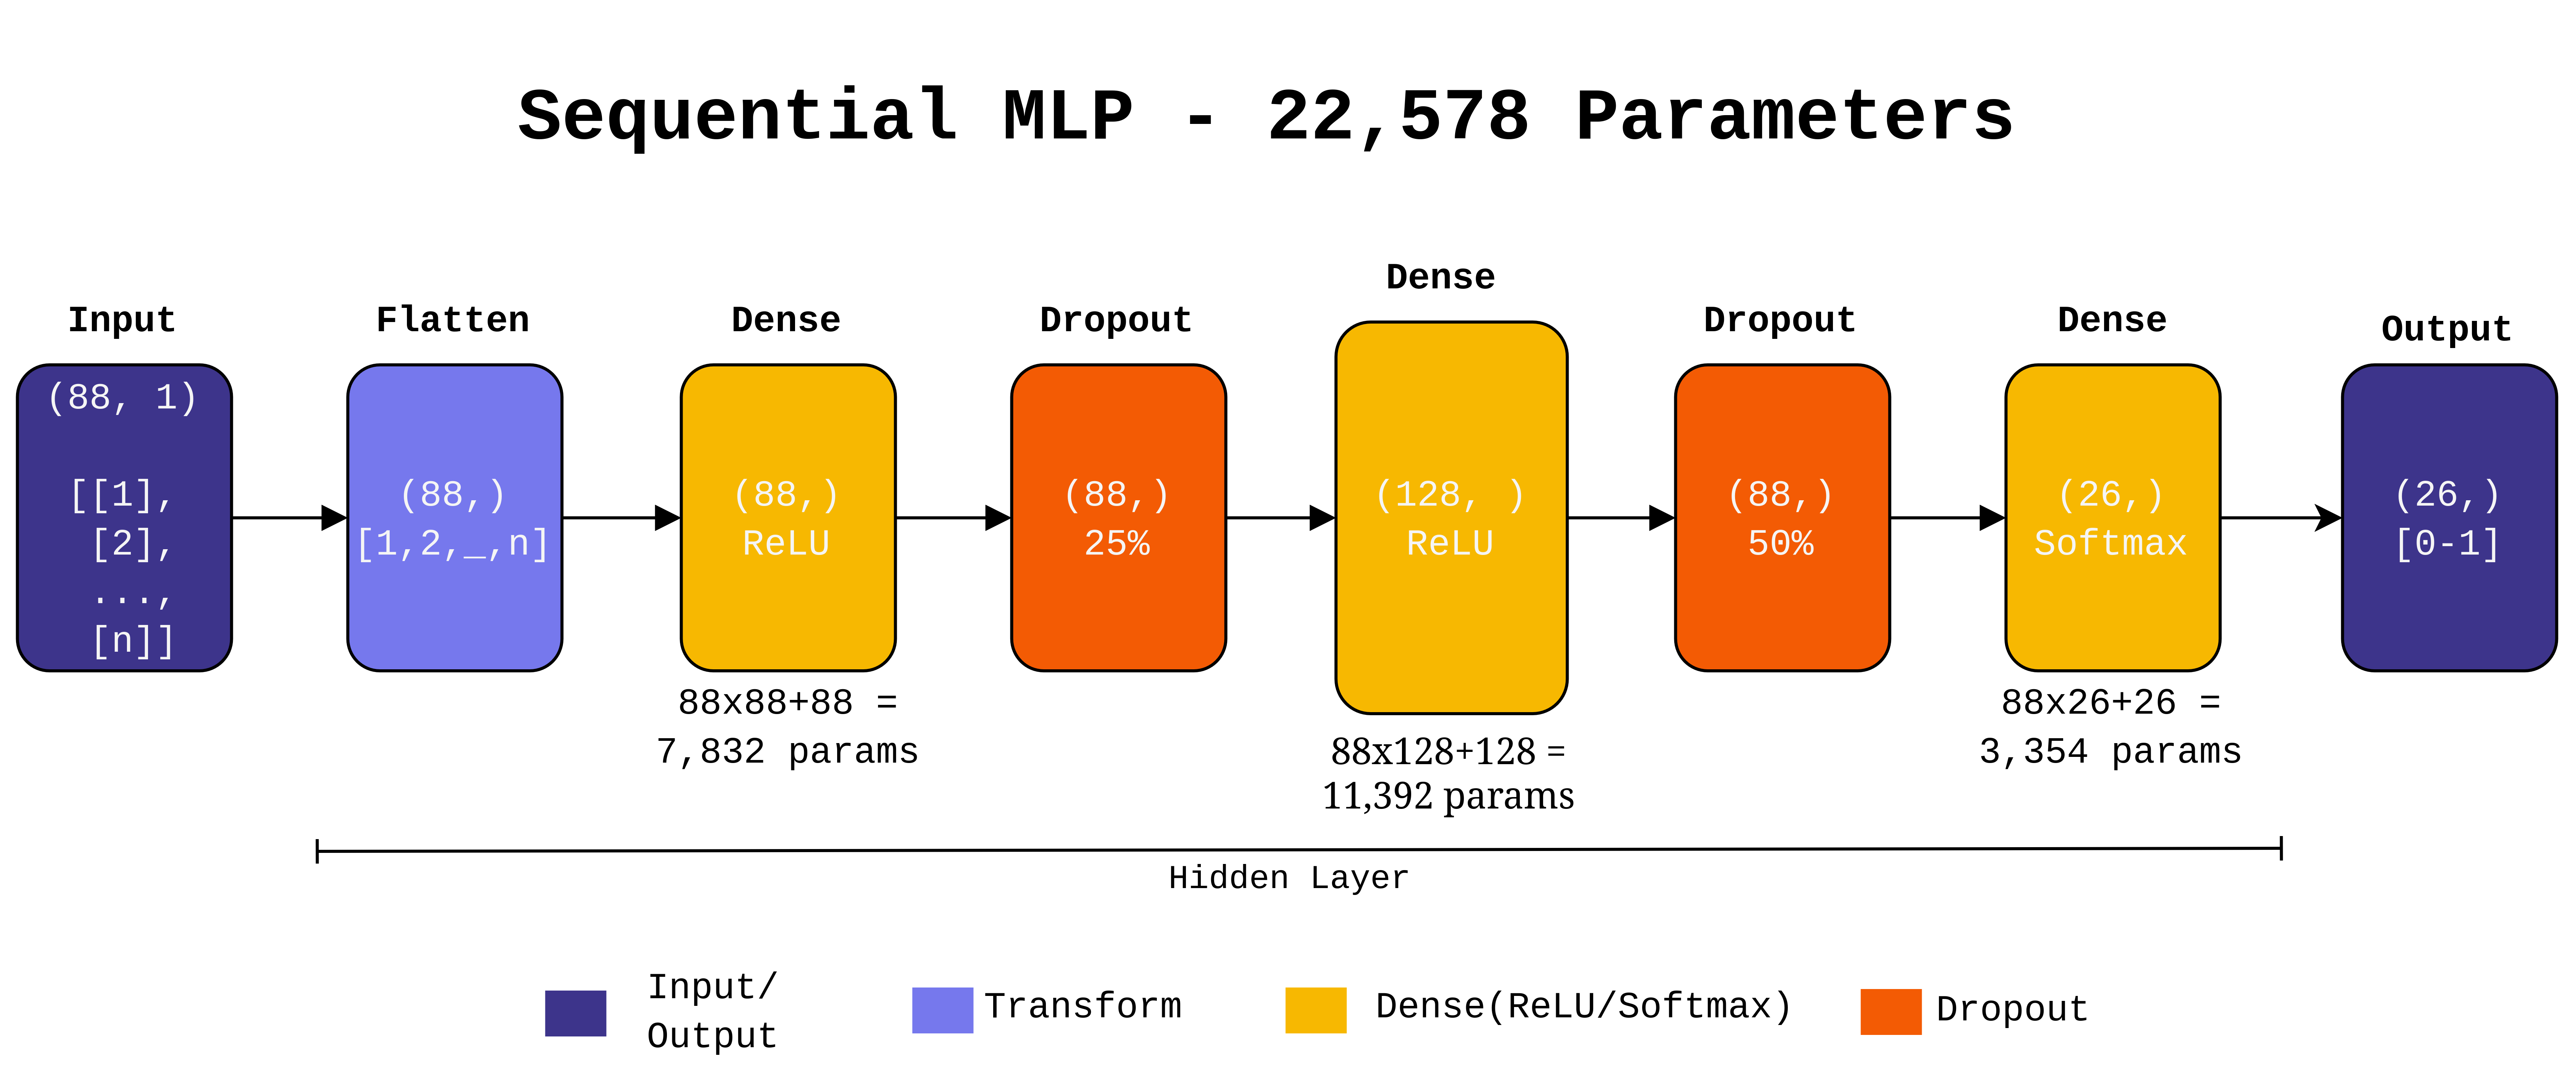
\includegraphics[width=0.8\textwidth]{material/figures/Sequential MLP.drawio.png}
    \caption{Architektur des Multi-Layer Perceptrons | Eigene Darstellung}
    \label{fig:mlp-architektur}
\end{figure}

Das Klassifikationsmodell setzt sich aus sieben Schichten zusammen, die sequenziell eine direkte Informationsflussrichtung von der Eingabe zur Ausgabe aufweisen. Die Architektur folgt dem Prinzip der schrittweisen Transformation und Abstraktion der Eingabemerkmale. Nachdem der Input-Tensor in eine eindimensionale Darstellung überführt wurde, transformiert die erste Dense-Schicht die Rohmerkmale in einen repräsentativen Feature-Raum. Die nachfolgende Dense-Schicht erweitert diesen Raum, um komplexere Inter-Feature-Beziehungen modellieren zu können. Zwischen den Dense-Schichten werden Dropout-Schichten eingebunden um Zufall in das Modell zu bringen, um Overfitting zu verhindern. Die finale Dense-Schicht projeziert die gelernten Repräsentationen auf die 26 Ausgabeklassen.

Der Input-Layer empfängt einen tensor der Form \texttt{(88,1)}. Dieser Tensor repräsentiert die normalisierten Merkmale zweier Hände mit je 44 Werten. Pro enthalten sind 21 MediaPipe-Hand-Landmarks jeweils als \texttt{(x,y)}-Koordinate sowie die absolute Handgelenkposition ebenfalls als \texttt{(x,y)}. Alle Koordianten sind Handgelenksrelativ normalisiert und auf den int15-Bereich skaliert, sodass der Input-Wertebereich [-1, 1] beträgt.

Der Flatten-Layer überführt den mehrdimensionalen Input-Tensor in einen eindimensionalen Vektor der Länge 88. Dense-Schichten erwarten als Eingabe einen flachen Vektor, sodass die räumliche Struktur des Tensors (2 Hände x 44 Werte) für die nachfolgende Gewichtsmatrix aufgelöst werden kann.

Der erste Dense-Layer mit 88 Neuronen und ReLU-Aktivierung führt per-Feature-Transformationen durch. Das bedeutet durch die  Gewichtsmatrix (88 × 88) und den Bias-Vektor wird jedes Eingabemerkmal einzeln transformiert. Die ReLU-Aktivierung ($f(x) = \max(0, x)$) fügt Nicht-Linearität hinzu und ermöglicht es dem Modell, nicht-triviale Muster in den Landmark-Daten zu erkennen. (Sharma et al., 2020) Die Wahl von 88 Neuronen hält die Kapazität zunächst auf gleicher Dimension wie der Input und zwingt das Modell, die Merkmale in einem äquivalenten Raum abzubilden, bevor eine Dimensionserweiterung erfolgt.

Der Dropout-Layer (0.25) deaktiviert während des Trainings zufällig 25\% der Ausgaben des vorherigen Dense-Layers. Jedes Neuron wir mit einer Wahrscheinlichkeit von 0.25 auf den Wert 0 gesetzt. Die Summe über alle Neuronen bleibt dabei Gleich. Dies verhindert die Ko-Adaptierung von Neuronen, bei der sich mehrere Neuronen auf ein einzelnes Eingabemuster spezialisieren und dadurch das Modell anfällig für Overfitting wird. (Ying, 2019)

Der zweite Dense-layer mit 128 Neuronen und ReLU-Aktivierung erweitert den Feature-Raum von 88 auf 128 Dimensionen. Durch die Erhöhung der Kapazität kann des Modell Inter-Feature-Beziehungen modellieren, die über die per-Feature-Transformationen des vorherigen Layers hinausgehen. Typische Beziehungen umfassen:

\begin{itemize}

    \item Intra-Hand-Abhängigkeiten: Korrelation zwischen benachbarten Landmarks des Selben fingers (z.B. die Auslenkung von PIP und DIP des Indexfingers), zwischen verschiedenen fingern einer Hand sowie  die Orientierung der Hand und deren Rotation basierend auf der Handflächen features.
    \item Inter-Hand-Beziehungen: Zusammenhänge zwischen den Landmarks beider Hände, die bei einhändigen Gesten durch symmetrische oder asymmetrische Konfigurationen entstehen können.
    \item Komplexe Muster: Nicht-lineare Kombinationen mehrerer Landmarks, die erst in der erweiterten Repräsentation als discriminative Merkmale erkennbar werden.
\end{itemize}

Der zweite Dropout-Layer (0.5) wendet eine stärkere Regularisierung an als der erste Dropout-Layer. Die Rate von 50\% ist bewusst höher gewählt, da der vorherige Dense-Layer mit 128 Neuronen eine größere Modellkapazität aufweist und die Gefahr des Overfitting steigt. Die stärkere Regularisierung vor der Ausgabeschicht stellt sicher, dass das Modell nur die robustesten Feature-Repräsentationen für die finale Klassifikation verwendet.

Der dritte Dense-Layer mit 26 Neuronen und Softmax-Aktivierung bildet die finale Klassifikationsschicht. Die 26 Ausgabeneuronen entsprechen den 26 Klassen (NONE, A–Y ohne J und Z, SCH). Die Softmax-Funktion $$\sigma(z_i) = \frac{e^{z_i}}{\sum e^{z_j}}$$normalisiert (Sharma et al., 2020). Die Rohausgaben (Logits) in Wahrscheinlichkeiten, deren Summe exakt 1 ergibt. Jedes Ausgabeneuron liefert damit die Wahrscheinlichkeit dafür, dass der Input der entsprechenden Gebärdensprache-Klasse angehört.

\subsection{Verlustfunktion und Optimierung}

Für das Training des Modells wird die Verlustfunktion Sparse Categorical Crossentropy verwendet. Diese eignet sich insbesondere, da die Zielklassen als Integer und nicht als One-Hot-Vektoren kodiert vorliegen. Dadurch wird der Speicherbedarf reduziert und gleichzeitig eine numerisch stabile Berechnung der Gradienten ermöglicht. Die Verlustfunktion berechnet die Abweichung zwischen den tatsächlichen Klassen und den durch die Softmax-Ausgabe vorhergesagten Klassenwahrscheinlichkeiten und lässt sich durch folgende Formel beschreiben:

$$L = -\log(p_{y_{true}})$$
(What Is Sparse Categorical Crossentropy, 10:49:00+00:00) wobei $p_{y_{true}}$ die vom Modell vorhergesagte Wahrscheinlichkeit der tatsächlichen Klasse bezeichnet.

\subsection{Trainingsprozess}

Um einen Trainingsprozess durchlaufen zu können müssen Hyperparameter bestimmt werden. Zentral sind Optimizer, Lernrate, Verlustfunktion, Epochen, Trainingssplit, Batch Size und Frühzeitiges Stoppen.

Der Adam-Optimizer (Adaptive Moment Estimation) kombiniert die Vorteile von Momentum und adaptiven Lernraten (RMSProp). Er berechnet für jeden Parameter individuelle Lernraten auf Basis des ersten und zweiten Moments der Gradienten. Dadurch konvergiert das Modell in der Regel schneller und stabiler als klassische Optimierungsverfahren wie Stochastic Gradient Descent (SGD). Insbesondere bei kleinen oder mittelgroßen Datensätzen sowie komplexen neuronalen Netzen liefert Adam häufig robuste Ergebnisse, da weniger aufwendige Hyperparameteranpassungen erforderlich sind. (A. G. et al., 2026)

Die Lernrate bestimmt die Größe der Aktualisierungsschritte während der Optimierung. Eine sehr kleine Lernrate von $10^{-5}$ reduziert das Risiko, das Minimum der Verlustfunktion zu überschreiten oder instabile Trainingsverläufe zu erzeugen. Der Nachteil einer geringeren Lernrate besteht in einer längeren Trainingsdauer, die jedoch durch eine stabilere Konvergenz ausgeglichen wird.

Als Verlustfunktion eignet sich Sparse Categorical Crossentropy für Mehrklassenklassifikationen, bei denen die Zielklassen als Ganzzahlen (z. B. 0, 1, 2, …) codiert sind. Im Gegensatz zur Categorical Crossentropy ist keine One-Hot-Kodierung der Labels erforderlich, wodurch Speicherbedarf und Vorverarbeitungsaufwand reduziert werden. Die Verlustfunktion misst die Abweichung zwischen den vorhergesagten Klassenwahrscheinlichkeiten und den tatsächlichen Klassen und liefert somit eine geeignete Optimierungsgrundlage für Klassifikationsaufgaben.

Die Sparse categorical Accuracy Metrik gibt den Anteil der korrekt klassifizierten Beispiele an und stellt damit eine leicht interpretierbare Leistungskennzahl dar. Da die Zielklassen als Integer vorliegen, passt sie direkt zur verwendeten Verlustfunktion SparseCategoricalCrossentropy. Während die Verlustfunktion zur Optimierung dient, ermöglicht die Accuracy eine intuitive Bewertung der Modellleistung während des Trainings und auf den Validierungsdaten.

Eine Epoche entspricht einem vollständigen Durchlauf des Trainingsdatensatzes. Die Wahl von 20 Epochen bietet dem Modell ausreichend Möglichkeiten, die zugrunde liegenden Muster zu erlernen, ohne die Trainingszeit unnötig zu verlängern. Da zusätzlich Early Stopping eingesetzt wird, dient dieser Wert als maximale Obergrenze. Das Training endet automatisch früher, sobald keine Verbesserung der Validierungsleistung mehr festgestellt wird.

Ein weiterer Hyperparameter ist die Aufteilung der Trainingsdaten in Training, Validation und Testdaten. Durch die Aufteilung des Datensatzes in 64\% Trainingsdaten, 16\% Validierungsdaten und 20\% Testdaten kann die Generalisierungsfähigkeit des Modells während des Trainings überprüft werden. Die Validierungsdaten werden nicht für das Lernen verwendet und ermöglichen daher eine unabhängige Beurteilung der Modellleistung.

Die Batch Size legt fest, wie viele Trainingsbeispiele gleichzeitig verarbeitet werden, bevor eine Aktualisierung der Modellgewichte erfolgt. Eine Batchgröße von 128 stellt einen guten Kompromiss zwischen Rechenleistung, Speicherbedarf und Trainingsstabilität dar. Größere Batches ermöglichen eine effizientere Nutzung von GPU Hardware dar und liefern stabilere Gradienten, während kleinere Batches zwar stärkeres Rauschen erzeugen, jedoch teilweise eine bessere Generalisierung fördern. Die gewählte Batchgröße bietet daher eine ausgewogene Balance zwischen Trainingsgeschwindigkeit und Modellqualität.

Early Stopping dient der Vermeidung von Overfitting, indem das Training automatisch beendet wird, sobald sich die Validierungsleistung über mehrere Epochen hinweg nicht mehr verbessert. Mit einer Patience von 3 werden kleinere Schwankungen der Validierungsverluste toleriert, bevor das Training gestoppt wird. Dadurch wird verhindert, dass unnötig lange trainiert wird oder das Modell beginnt, sich zu stark an die Trainingsdaten anzupassen. Gleichzeitig wird das Modell mit der besten Validierungsleistung gespeichert bzw. verwendet.

\begin{longtable}{|p{0.35\textwidth}|p{0.55\textwidth}|}
    \caption{Hyperparameter des Modelltrainings}
    \label{tab:hyperparameter} \\
    \hline
    \textbf{Parameter} & \textbf{Wert} \\
    \hline
    \endfirsthead
    \hline
    \textbf{Parameter} & \textbf{Wert} \\
    \hline
    \endhead
    \hline
    \multicolumn{2}{r}{\textit{Fortsetzung auf nächster Seite}} \\
    \endfoot
    \hline
    \endlastfoot
    Optimizer & Adam \\
    \hline
    Learning Rate & 0,00001 \\
    \hline
    Verlustfunktion & Sparse Categorical Crossentropy \\
    \hline
    Metrik & Sparse Categorical Accuracy \\
    \hline
    Epochen & 20 \\
    \hline
    Validation Split & 0,2 (80/20) \\
    \hline
    Batch Size & 128 \\
    \hline
    Early Stopping & 3 \\
    \hline
\end{longtable}

\subsection{Evaluierung}

Die Evaluierung der Ergebnisse des Machine Learning Modells sind in Kapitel 8 zu finden.
\#TODO Füge kapitelreferenz ein!

\section{Quantisierung, Konvertierung und Deployment der Modelle}

Das folgende Kapitel beschreibt die Quantisierung des Tensorflow Fingeralphabet Modells, die Convertierung der Quantisierten Handdedektion-, Landmarkerkennung- und Fingeralphabet- Modelle in NPU ausführbare Binaries. Im letzten Schritt wird das Flashen der Modelle auf den STM32N650DK beschrieben.

\subsection{Quantisierung von Tensorflow Modellen}

a die Modelle zur Handdetektion und Landmark-Erkennung bereits in einer quantisierten Form vorliegen, ist für diese keine weitere Quantisierung erforderlich. Lediglich das Modell zur Erkennung des Fingeralphabets muss für den Einsatz auf der Zielhardware quantisiert werden. Die Quantisierung erfolgt im Rahmen der Konvertierung des trainierten Keras-Modells in das TensorFlow-Lite-Format (TFLite). Dieser Schritt ist notwendig, da die Generierung der Embedded-Binärdateien mit STEdgeAI ausschließlich Modelle im TensorFlow-Lite- oder ONNX-Format unterstützt.

Bei der Konvertierung wird eine Post-Training-Quantisierung (PTQ) durchgeführt. Hierbei werden die Gewichte und Aktivierungen des bereits trainierten Modells von Gleitkommazahlen (Float32) auf 8-Bit-Ganzzahlen (INT8) abgebildet. Da die eingesetzte Neural Processing Unit (NPU) ausschließlich vollständig INT8-quantisierte Modelle unterstützt, müssen sowohl die internen Operationen als auch die Ein- und Ausgabedaten des Modells diesem Format entsprechen.

Zunächst wird das trainierte Keras-Modell geladen und ein Tensorflow-Lite-Konverter erzeugt.

\begin{lstlisting}[language=python, caption={TensorFlow-Lite Konverter erzeugen}, label={lst:tflite-converter}]
model = keras.models.load_model(MODEL_DIR)
converter = tf.lite.TFLiteConverter.from_keras_model(model)
\end{lstlisting}

Anschließend werden die Standardoptimierungen des Konverters aktiviert:

\begin{lstlisting}[language=python, caption={Optimierung aktivieren}, label={lst:tflite-optimization}]
converter.optimization = [tf.lite.Optimize.DEFAULT]
\end{lstlisting}

Für die Kalibrierung der Quantisierung wird ein repräsentativer Datensatz bereitgestellt:

\begin{lstlisting}[language=python, caption={Repräsentativer Datensatz}, label={lst:tflite-representative}]
converter.representative_dataset = representative_dataset
\end{lstlisting}

Während der Kalibrierung bestimmt TensorFlow Lite anhand dieser Daten die Wertebereiche der Aktivierungen, um geeignete Skalierungsfaktoren und Nullpunkte für die Quantisierung zu berechnen. Sind die Trainingsdaten nicht verfügbar, wird ersatzweise ein Datensatz aus gleichverteilten Zufallswerten im Bereich `[-1, 1]` verwendet.

Da die Zielhardware ausschließlich INT8-Operationen unterstützt, wird die Konvertierung entsprechend eingeschränkt und zusätzlich die Ein- und Ausgabedatentyp des Modells auf 8-Bit-Ganzzahlen festgelegt:
\begin{lstlisting}[language=python, caption={INT8-Quantisierung konfigurieren}, label={lst:tflite-int8}]
converter.target_spec.supported_ops = [
    tf.lite.OpsSet.TFLITE_BUILTINS_INT8
]

converter.inference_input_type = tf.uint8
converter.inference_output_type = tf.uint8
\end{lstlisting}

Abschließend wird das Modell in das Tensorflow-Lite-Format konvertiert und als \texttt{.tflite-Datei} gespeichert.

Ergebnis ist ein vollständig quantisiertes TensorFlow-Lite-Modell, das den Anforderungen der eingesetzten NPU entspricht und anschließend mit STEdgeAI in eine für das Embedded-System ausführbare Binärdatei überführt werden kann. Durch die Quantisierung werden der Speicherbedarf und der Rechenaufwand reduziert, während die Modellgenauigkeit durch die Verwendung repräsentativer Kalibrierungsdaten weitgehend erhalten bleibt.

\subsection{Konvertierung INT8-Quantisierte-Modelle zu Embedded binaries}

Nach der Quantisierung liegen alle drei Modelle (Handdetektion, Handlandmark-Erkennung und Fingeralphabet-Klassifikation) im TensorFlow-Lite-Format mit einer INT8-Quantisierung vor. Der nächste Verarbeitungsschritt ist diese Modelle mithilfe der ST Edge AI Core CLI in für die Zielhardware ausführbare Binärdateien zu überführen. Die Verwendung der Kommandozeilenschnittstelle (CLI) wurde bewusst der grafischen Benutzeroberfläche (GUI) vorgezogen, da sich hierdurch der gesamte Konvertierungsprozess automatisieren lässt. Auf diese Weise können Skripte erstellt werden, welche die Generierung aller Modellartefakte reproduzierbar und mit einem einzelnen Aufruf durchführen.

Die Verzeichnisstruktur der Modellgenerierung:

\begin{lstlisting}[language=bash, numbers=none, caption={Verzeichnisstruktur der Modellgenerierung}, label={lst:model-dir-structure}]
models/
+-- source/                           <- Raw TFLite models (input)
|   +-- 033_palm_detection_full_quant_pc_ff_od.tflite
|   +-- 033_hand_landmark_full_quant_pc_uf_handl.tflite
|   \-- fingeralphabet_model_int8.tflite
|
+-- my_mpools/                        <- Memory pool definitions per model
|   +-- palm_detection.mpool
|   +-- hand_landmark.mpool
|   \-- fingeralphabet.mpool
|
+-- user_neuralart.json   <- Per-model config (links model -> mpool+compiler flags)
+-- generate_n6_models.sh <- Orchestrator script (calls stedgeai, copies outputs)
+-- copy_n6_models.sh     <- Copies generated files into the firmware project tree
|
+-- generated/            <- Output: C source + headers ready for compilation
|   +-- palm/
|   +-- landmark/
|   \-- finger/
|
\-- st_ai_output/         <- Intermediate build artifacts (gitignored)
\end{lstlisting}

\paragraph{Modell Profile}

In der Struktur definiert \texttt{user\_neuralart.json} wie die einzelnen Modelle bei der Compilierung für die STM32N6 NPU zu behandeln sind. Sie enthält einen Abschnitt \texttt{Profiles} mit jeweils einem Eintrag pro Modell:

\begin{lstlisting}[language=json, caption={Modellprofil in user\_neuralart.json}, label={lst:user-neuralart}]
{
  "Profiles": {
    "palm_detection_model_v3": {
      "memory_pool": "./my_mpools/palm_detection.mpool",
      "options": "--enable-epoch-controller"
                 "-O3"
                 "--all-buffers-info"
                 "--cache-maintenance"
    }
  }
}
\end{lstlisting}

\texttt{memory\_pool} \newline
Verweist auf die \texttt{.mpool}-Datei, die das Speicherlayout der NPU für dieses Modell definiert (welche SRAM-Bänke, Flash-Bereiche, Adressen und Größen).

\texttt{options} \newline
Definiert pro Modell welche Compilerflags verwendet werden sollen. Folgend werden verwendete Compiler flags in \ref{tab:tab:stedgeai-flags} kurz erläutert.

\begin{longtable}{|p{0.32\textwidth}|p{0.63\textwidth}|}
    \caption{ST Edge AI Core Compiler Flags}
    \label{tab:stedgeai-flags} \\
    \hline
    \textbf{Flag} & \textbf{Effekt} \\
    \hline
    \endfirsthead
    \hline
    \textbf{Flag} & \textbf{Effekt} \\
    \hline
    \endhead
    \hline
    \multicolumn{2}{r}{\textit{Fortsetzung auf nächster Seite}} \\
    \endfoot
    \hline
    \endlastfoot
    --enable-epoch-controller & Ermöglicht die epochenbasierte Ausführung der NPU (schichtweise Ablaufplanung) \\
    \hline
    -O3/-O2 & Optimierungsstufe für den NPU-Codegenerator \\
    \hline
    --all-buffers-info & Vollständige Puffer-Metadaten für die Laufzeit ausgeben \\
    \hline
    --cache-maintenance / --Ocache-opt & Befehle zum Leeren/Ungültigmachen des Caches einfügen \\
    \hline
    --Oauto-sched & Automatisches planen der Epochen (default/Ohne Verweis) \\
    \hline
    --native-float & Verwendet Hardware-Float-Operationen wenn möglich \\
    \hline
    --enable-virtual-mem-pools & Erlaubt dem Linker Tensoren über mehrere physische Speicherregionen zu verteilen \\
    \hline
    --Omax-ca-pipe \texttt{<num>} & Legt die maximale Anzahl an Compute-\&-Accumulate-(CA-)Pipelines bzw.\ parallelen Hardware-Ausführungspfaden fest, die der Compiler gleichzeitig zuweisen darf. \\
    \hline
    --Oconv-split-kw & Aufteilen von Faltungskernen auf die verfügbaren NPU-MAC-Arrays \\
    \hline
\end{longtable}

\paragraph{Memory-Pool-Definition}
Die \texttt{.mpool}-Dateien beschreiben die STM32N6 Hardware Speicherabbild der NPU. Alle \texttt{.mpool}-Dateien haben den identischen Aufbau. Der einzige wesentliche Unterschied zwischen den Modellen besteht in der xSPI2 (flash) Region (Basisadresse und Größe) an welcher die Modelle gespeichert sind.

Hauptbereiche:

\texttt{params}

\begin{lstlisting}[language=json, caption={Globale Speicher einschränkung in .mpool}, label={lst:mpool-params}]
{ "paramname": "max_onchip_sram_size", "value": "1024", "magnitude": "KBYTES"}
\end{lstlisting}

Beschränkt die maximale verfügbare On-Chip-SRAM-Größe auf 1024\,KB für die NPU.

\texttt{cacheinfo} Beschreibt den Cache.

\texttt{mempools} Speicherbereich-Konfiguration pro Modell auf der NPU.

\begin{longtable}{|l|l|l|l|p{0.3\textwidth}|}
    \caption{NPU-Speicherbereich-Konfiguration}
    \label{tab:npu-mempools} \\
    \hline
    \textbf{Name} & \textbf{Region} & \textbf{Adresse} & \textbf{Größe} & \textbf{Rolle} \\
    \hline
    \endfirsthead
    \hline
    \textbf{Name} & \textbf{Region} & \textbf{Adresse} & \textbf{Größe} & \textbf{Rolle} \\
    \hline
    \endhead
    \hline
    \multicolumn{5}{r}{\textit{Fortsetzung auf nächster Seite}} \\
    \endfoot
    \hline
    \endlastfoot
    npuRAM3 & AXISRAM3 & 0x34200000 & 448\,KB & NPU activation scratch \\
    \hline
    npuRAM4 & AXISRAM4 & 0x34270000 & 448\,KB & NPU activation scratch \\
    \hline
    npuRAM5 & AXISRAM5 & 0x342e0000 & 448\,KB & NPU activation scratch \\
    \hline
    npuRAM6 & AXISRAM6 & 0x34350000 & 448\,KB & NPU activation scratch \\
    \hline
    hyperRAM & xSPI1 & 0x90000000 & 0\,MB & External HyperRAM (Deaktiviert) \\
    \hline
    octoFlash & xSPI2 & 0x71000000 & 2\,MB & Weight storage in OctoSPI flash \\
    \hline
\end{longtable}

Die vier AXISRAM-Bänke sind On-Chip-SRAM-Speicher mit hohem Durchsatz und geringer Latenz, die für Laufzeit-Aktivierungen (Zwischentensoren) genutzt werden. \texttt{octoFlash} ist zur Laufzeit schreibgeschützt (ACC\_READ) und speichert die Modellgewichte bzw.\ -konstanten. Die Einstellung \texttt{constants\_preferred: "true"} weist das Tool an, konstante Daten in diesem Bereich abzulegen.

Die Flash-Basisadressen unterscheiden sich je nach Modell, um den 16-MB-xSPI2-Flash zu partitionieren:

\begin{longtable}{|l|l|l|}
    \caption{Flash-Partitionierung je Modell}
    \label{tab:flash-partitionierung} \\
    \hline
    \textbf{Modell} & \textbf{Flash Start} & \textbf{Flash Size} \\
    \hline
    \endfirsthead
    \hline
    \textbf{Modell} & \textbf{Flash Start} & \textbf{Flash Size} \\
    \hline
    \endhead
    \hline
    \multicolumn{3}{r}{\textit{Fortsetzung auf nächster Seite}} \\
    \endfoot
    \hline
    \endlastfoot
    Finger & 0x71000000 & 2\,MB \\
    \hline
    Handdetektion & 0x71200000 & 4\,MB \\
    \hline
    Handlandmark & 0x71600000 & 10\,MB \\
    \hline
\end{longtable}

\paragraph{Script - Generierung}
Das \texttt{generate\_n6\_models.sh}-Script führt für jedes Modell 3 Schritte durch (Konvertierung, Kopieren und Project-Build).

Im ersten Schritt wird die ST Edge AI core CLI zur konvertierung \texttt{TF-Lite $\rightarrow$ NPU-Artefakte} verwendet.

\begin{lstlisting}[language=bash, caption={STedgeAI Modellgenerierung}, label={lst:stedgeai-generate}]
stedgeai generate \
    --name palm_detection_model_v3 \
    --model source/033_palm_detection_full_quant_pc_ff_od.tflite \
    --target stm32n6 \
    --st-neural-art "palm_detection_model_v3@user_neuralart.json" \
    --input-data-type uint8 \
    --output st_ai_output/
\end{lstlisting}

Dies liest das TensorFlow-Lite-Modell ein, lädt die \texttt{palm\_detection\_model\_v3} Konfiguration in \texttt{user\_neuralart.json} um den Memory-Pool und Compiler-Optionen zu erhalten und generiert:
\begin{itemize}
    \item Eine \texttt{.c}-Datei mit Gewichtsdaten als C-Arrays (die rohen Binärdaten sind eingebettet)
    \item Ein Header namens \texttt{\_ecblobs.h}, der diese Arrays mit Attributen für Linker-Sektionen deklariert
    \item \texttt{stai\_\*.c} / \texttt{stai\_\*.h} -- der ST-AI-Runtime-API-Wrapper (Zuweisung, Laden, Ausführung der Inferenz)
    \item Ein \texttt{\*\_atonbuf.xSPI2.raw} file -- Der Binär-Blob mit den Gewichten für die Flash-Programmierung
\end{itemize}

Der zweite Schritt Konvertiert \texttt{.raw} Gewichts-Blob in eine Intel \texttt{.hex}-Datei mit der korrekten Basisadresse (z.\,B.\ 0x71000000). Diese Hex-Datei kann via STM32CubeProgrammer auf den Mikrocontroller geflashed werden.

Der lertzte Schritt führt das \textttt{copy\_n6\_models.sh}-Script aus es kopiert die generierten Dateien in das STM32N6570DK-Embedded-Projekt:
\begin{itemize}
    \item \texttt{*.c} und \texttt{*\_ecblobs.h} $\rightarrow$ \texttt{embedded/STM32N6570DK/FSBL/Src/AI/\textless Model\textgreater/Src/Inc/}
    \item \texttt{stai\_\*.c/h} (with \texttt{--stai} flag)
    \item \texttt{*.bin} weight blobs (with \texttt{--weights} flag) $\rightarrow$ \texttt{FSBL/Assets/AI/}
\end{itemize}

Zudem wird \texttt{\*\_ecblobs.h} gepatcht, um \texttt{\#include "ecblob\_sections.h"} einzufügen. Dadurch wird sichergestellt, dass die Gewichts-Arrays im ECBLOBS-Linker-Abschnitt (0x72000000, 8\,MB) landen, anstatt des internen ROM (255\,KB) zu sprengen.

\section{Softwaregrundstruktur und hardwarenahe Basistreiber}
\subsection{Aufbau der Embedded-Software}

Die Embedded-Software ist in einem modularen Verzeichnisbaum organisiert. Die wesentlichen Komponenten sind:

\begin{lstlisting}[language=bash, numbers=none, caption={Verzeichnisstruktur der Embedded-Software}, label={lst:sw-dir-structure}]
STM32N6570DK/
+-- Appli/                    <- Applikation (Appli-Projekt)
|   \-- Src/
|       \-- main.c            <- Applikations-Einstiegspunkt
|
\-- FSBL/                     <- First Stage Bootloader
    \-- Src/
        +-- AI/               <- KI-Modelle und Verarbeitung
        |   +-- Base/         <- Generische KI-Schnittstelle
        |   +-- Fingeralphabet/  <- Fingeralphabet-Klassifikation
        |   +-- Hand_landmark/   <- Hand-Landmark-Erkennung
        |   \-- Palm_detection/  <- Handflaechen-Detektion
        |
        +-- Assets/           <- Bildmaterial (Bitmaps)
        +-- Core/             <- Systemkonfiguration und Ablaufsteuerung
        |   +-- main.c        <- Einstiegspunkt
        |   +-- app.c         <- Hardware-Init-Koordination
        |   +-- config.c      <- Zentrale Konfigurationsstrukturen
        |   \-- tasks.c       <- Scheduler-Aufgaben
        |
        +-- Drivers/          <- Treiberschicht
        |   +-- CMSIS/        <- Arm CMSIS-Bibliothek
        |   +-- HAL/          <- ST HAL-Bibliothek
        |   \-- Simple/       <- Projektspezifische Treiber
        |       +-- Src/      <- Implementierungen
        |       \-- Inc/      <- Oeffentliche Schnittstellen
        |
        \-- Middlewares/      <- Externe Bibliotheken
            \-- ST/AI/        <- ST Neural-ART NPU-Middleware
\end{lstlisting}

\subsection{Zentrale Konfiguration und Systeminitialisierung}

Die zentrale Konfiguration bündelt alle Hardware-Einstellungen an einem Ort. Konfigurationsstrukturen werden als konstante Arrays definiert und dem jeweiligen Treiber bei der Initialisierung übergeben:

\begin{lstlisting}[language=c, caption={GPIO-Konfigurationsstrukturen}, label={lst:gpio-config-struct}]
const GPIO_cfg_TypeDef GPIO_LTDC_cfg = {
    .mode   = GPIO_MODE_AF,
    .otyp   = GPIO_OTYPE_PP,
    .pupdr  = GPIO_PUPD_UP,
    .af     = GPIO_AF_LTDC,
    .speed  = GPIO_SPEED_VERY_HIGH
};

const GPIO_cfg_TypeDef GPIO_I2C_cfg = {
    .mode   = GPIO_MODE_AF,
    .otyp   = GPIO_OTYPE_OD,
    .pupdr  = GPIO_PUPD_UP,
    .af     = GPIO_AF_I2C,
    .speed  = GPIO_SPEED_HIGH
};
\end{lstlisting}

Durch die Verwendung von \texttt{const}-Qualifizern werden die Konfigurationsstrukturen im Flash-Speicher abgelegt und verbrauchen keine SRAM-Ressourcen. Die benannten Initialisierer (\texttt{.mode}, \texttt{.af}, etc.) machen den Code lesbar und fehlerresistenter.

\subsection{Registerbasierte Treiberentwicklung}

Für die hardwarenahe Treiberentwicklung werden Peripherie-Einheiten über Memory-Mapped I/O-Register konfiguriert. Das folgende Beispiel zeigt einen GPIO-Treiber, der die Modus-, Ausgabe- und Pull-Up/Pull-Down-Konfiguration eines Pins über direkte Bitmanipulation an den GPIO-Registern setzt:

\begin{lstlisting}[language=c, caption={Registerbasierte GPIO-Konfiguration}, label={lst:gpio-config}]
void GPIO_Config(GPIO_TypeDef *GPIOX, uint32_t pinNr,
                 GPIO_cfg_TypeDef cfg){
    RCC_enable_GPIO(GPIOX);
    GPIOX->MODER  = (GPIOX->MODER  & ~(3U << (2U * pinNr)))
                    | (cfg.mode  << (2U * pinNr));
    GPIOX->OTYPER = (GPIOX->OTYPER & ~(1U << (pinNr)))
                    | (cfg.otyp  << (pinNr));
    GPIOX->PUPDR  = (GPIOX->PUPDR  & ~(3U << (2U * pinNr)))
                    | (cfg.pupdr << (2U * pinNr));

    if (cfg.mode == GPIO_MODE_AF) {
        GPIO_set_af(GPIOX, pinNr, cfg.af, cfg.speed);
    }
}
\end{lstlisting}

Die Bitmanipulation folgt dem typischen Muster: Bestehende Bits werden mit einer Maske gelöscht (\texttt{\& \textasciitilde mask}) und anschließend werden die neuen Werte gesetzt (\texttt{| value}). Die Makro \texttt{(2U * pinNr)} berechnet die Bitposition, da jedes GPIO-Register 2 Bits pro Pin reserviert.

\subsection{Grundlegende Systemtreiber}
\subsection{Einordnung der Basistreiber in die übergeordneten Komponenten}

\section{Kamera - Display Pipeline}
Text.

\subsection{Initialisierung des Kamerasensors}
\subsection{Übertragung der Kameradaten über CSI und DCMIPP}
\subsection{Verwaltung der Bildpuffer}
\subsection{LTDC-Konfiguration und Verwaltung der Displayebenen}

\section{Ablaufsteuerung und Software Scheduler}

\section{Integration der NPU und einheitliche KI-Schnittstelle}
\subsection{Initialisierung des Neural-ART Accelerators}
\subsection{Einheitliche KI-Schnittstelle}

\section{Vor- und Nachverarbeitungsschritte}
\subsection{DCMIPP-gestützte Bildvorverarbeitung}
\subsection{Nachverarbeitung der Handdetektion}
\subsection{Vorverarbeitung der Landmark-Erkennung}
\subsection{Nachverarbeitung der Landmark-Erkennung}
\subsection{Vorverarbeitung des Klassifizierungsmodells}
\subsection{Nachverarbeitung des Klassifikationsmodells}

\section{Visualisierung und Benutzerausgabe}
\subsection{Darstellung der Erkennungsergebnisse}
\subsection{Benutzeroberfläche und Bedienung}

\section{Optimierungen}
